% !TeX program = pdflatex
% !BIB program = biber
% !TeX root = main.tex
% =============================================================================
% MAIN.TEX — Master document for the ANU MAE Thesis
% =============================================================================
%
% This file controls the overall structure of your thesis.
% Write your chapter content in the individual .tex files, not here.
%
% HOW TO COMPILE
%   Overleaf:   click Recompile (Menu → Compiler → pdfLaTeX)
%   TeXstudio:  press F5 (Build & View) — see README for one-time setup
%   Terminal:   latexmk main.tex
%
% =============================================================================

% =============================================================================
% DOCUMENT FORMAT — activate ONE option by removing the leading %
% Also update the matching geometry line in preamble.tex (same option number).
% =============================================================================
%
% OPTION 1 — Digital submission (default)
%   All margins 2.5 cm. Single-sided layout.
\documentclass[a4paper, 11pt, oneside]{book}
%
% OPTION 2 — Hard copy, single-sided printing
%   Wider left margin for binding. See preamble.tex Option 2 for margins.
% \documentclass[a4paper, 11pt, oneside]{book}
%
% OPTION 3 — Hard copy, double-sided printing
%   Wider inner (binding) margin on every page. See preamble.tex Option 3 for margins.
% \documentclass[a4paper, 11pt, twoside]{book}
%
% =============================================================================

% ===================== Compiler =====================
% This template uses pdfLaTeX (the default Overleaf compiler).
% In Overleaf: Menu → Compiler → pdfLaTeX
% Locally: run `latexmk main.tex` (see README and latexmkrc)

% ===================== Core Packages =====================
\usepackage[T1]{fontenc}
\usepackage[utf8]{inputenc}

% Pre-register xcolor options so makecell loading xcolor later doesn't warn
\PassOptionsToPackage{table,xcdraw}{xcolor}

% Declare Unicode characters that may appear in bibliography titles/fields
% so pdfLaTeX does not error on them (Greek letters, math symbols).
\DeclareUnicodeCharacter{03B1}{\ensuremath{\alpha}}   % α
\DeclareUnicodeCharacter{03B2}{\ensuremath{\beta}}    % β
\DeclareUnicodeCharacter{03B3}{\ensuremath{\gamma}}   % γ
\DeclareUnicodeCharacter{03BC}{\ensuremath{\mu}}      % μ (Greek mu, distinct from µ micro)
\DeclareUnicodeCharacter{2265}{\ensuremath{\geq}}     % ≥
\DeclareUnicodeCharacter{2264}{\ensuremath{\leq}}     % ≤
\DeclareUnicodeCharacter{2212}{\ensuremath{-}}        % − (minus sign)
\DeclareUnicodeCharacter{F6D9}{\relax}                % private-use glyph in some PDF paths

% Activate the geometry line that matches your chosen option in main.tex.
% OPTION 1 — Digital submission: all margins 2.5 cm
\usepackage[a4paper, margin=2.5cm]{geometry}
% OPTION 2 — Hard copy, single-sided: left 4 cm (binding), top/right/bottom 2 cm
% \usepackage[a4paper, left=4cm, top=2cm, right=2cm, bottom=2cm]{geometry}
% OPTION 3 — Hard copy, double-sided: inner 4 cm (binding), outer/top/bottom 2 cm
% \usepackage[a4paper, inner=4cm, outer=2cm, top=2cm, bottom=2cm]{geometry}

\usepackage{ragged2e}
\usepackage[none]{hyphenat}
\usepackage{microtype}
\usepackage{titlesec}
\usepackage[english]{babel}
\usepackage{xurl}
\emergencystretch=3em
\setlength{\parindent}{0pt}
\setlength{\parskip}{1em}
\RaggedRight

% ===================== Fonts =====================
% Helvetica — visually equivalent to Arial, compatible with pdfLaTeX
\usepackage[scaled]{helvet}
\renewcommand\familydefault{\sfdefault}

% ===================== Graphics and Layout =====================
\usepackage{graphicx}
\usepackage{rotating}
\usepackage{pdfpages}
\usepackage{emptypage}
\usepackage{needspace}
\usepackage{adjustbox}
\usepackage{pdflscape}
\usepackage{afterpage}
\graphicspath{ {figures/} }

% ===================== Floats and Tables =====================
\usepackage{threeparttable}
\usepackage{float}
\usepackage{multirow}
\usepackage{xcolor}
\usepackage{makecell}
\usepackage{array}
\renewcommand{\arraystretch}{1.2}

% ===================== Captions =====================
\usepackage[font=it,justification=raggedright,singlelinecheck=false,hypcap=false]{caption}
\setlength{\abovecaptionskip}{4pt}
\setlength{\belowcaptionskip}{4pt}

\DeclareCaptionType{textbox}[Box][List of boxes]

% ===================== TOC and Lists =====================
\usepackage[nottoc,notlof,notlot]{tocbibind}
\usepackage[title,titletoc]{appendix}
\usepackage{etoc}

\renewcommand{\contentsname}{Table of Contents}
\renewcommand{\listfigurename}{List of Figures}
\renewcommand{\listtablename}{List of Tables}

% --- Make TOC chapter entries bold ---
\makeatletter
\renewcommand*{\l@chapter}[2]{%
  \addpenalty{-\@highpenalty}%
  \vskip 1.0em
  \@dottedtocline{0}{0em}{3em}{\bfseries #1}{\bfseries #2}%
}
\makeatother

% --- Section formatting in TOC ---
\makeatletter
\renewcommand*\l@section[2]{%
  \vspace{0.4em}%
  \@dottedtocline{1}{1.5em}{3.2em}{\bfseries #1}{\bfseries #2}%
}
% Subsection numbers start level with the section name (indent = 1.5em + 3.2em = 4.7em)
\renewcommand*\l@subsection[2]{%
  \@dottedtocline{2}{4.7em}{3.2em}{#1}{#2}%
}
\makeatother

% --- Hide Contents from TOC itself but add PDF bookmark ---
\let\temptableofcontents\tableofcontents
\renewcommand{\tableofcontents}{
  \renewcommand{\contentsname}{Table of contents}
  \cleardoublepage
  \pdfbookmark[0]{\contentsname}{toc}
  \temptableofcontents
}

% Set up etoc depth tags for chapters vs appendices
\etocsettagdepth{mtchapter}{subsection}
\etocsettagdepth{mtappendix}{none}

% Local table of contents (one per chapter)
\newcommand{\localtoc}{%
  \etocsettocstyle{\section*{Table of contents}}{}
  \begingroup
  \setlength{\parskip}{1pt}
  \etocsetnexttocdepth{subsection}
  \localtableofcontents
  \endgroup
}

% ── Per-chapter local figure / table lists ─────────────────────────────────
% Strategy: mirror each lof/lot \addcontentsline call into the .toc file as
% custom 'lofitem'/'lotitem' entries. \locallistoffigures / \locallistoftables
% read those back per-chapter via etoc's \localtableofcontents.
%
% The patch is installed via \AddToHook{begindocument/end} — which fires after
% ALL other begindocument hooks (including hyperref's), so we capture the truly
% final \addcontentsline.  Using \edef expands the file-extension argument
% before comparison so the \ifx test works correctly even when the argument is
% a \csname...\endcsname token.  The hook body contains NO # characters,
% avoiding the LaTeX 2025 L3 hook issue where ## is not halved to #.

\etocsetlevel{lofitem}{5}
\etocsetlevel{lotitem}{5}

\renewcommand{\locallistoffigures}{%
  \begingroup
  \etocsettagdepth{mtchapter}{5}%
  \etocsetlevel{lotitem}{6}%     % push tables to etoc's "never shown" sentinel depth
  \etocsetlevel{lofitem}{5}%     % keep figures at depth 5
  \RaggedRight
  \setlength{\parskip}{0.5em}
  \etocsettocstyle{\section*{List of figures}}{}%
  \etocsetstyle{chapter}{}{}{}{}%
  \etocsetstyle{section}{}{}{}{}%
  \etocsetstyle{subsection}{}{}{}{}%
  \etocsetstyle{subsubsection}{}{}{}{}%
  \etocsetstyle{paragraph}{}{}{}{}%
  \etocsetstyle{subparagraph}{}{}{}{}%
  \etocsetstyle{lofitem}{}{}{\noindent\hangindent=2.5em\hangafter=1\etoclink{\makebox[2.5em][l]{\etocnumber}\etocname}\dotfill\etocthelinkedpage\par}{}%
  \etocsetnexttocdepth{5}%
  \localtableofcontents
  \endgroup
}

\renewcommand{\locallistoftables}{%
  \begingroup
  \etocsettagdepth{mtchapter}{5}%
  \etocsetlevel{lofitem}{6}%     % push figures to etoc's "never shown" sentinel depth
  \etocsetlevel{lotitem}{5}%     % keep tables at depth 5
  \RaggedRight
  \setlength{\parskip}{0.5em}
  \etocsettocstyle{\section*{List of tables}}{}%
  \etocsetstyle{chapter}{}{}{}{}%
  \etocsetstyle{section}{}{}{}{}%
  \etocsetstyle{subsection}{}{}{}{}%
  \etocsetstyle{subsubsection}{}{}{}{}%
  \etocsetstyle{paragraph}{}{}{}{}%
  \etocsetstyle{subparagraph}{}{}{}{}%
  \etocsetstyle{lotitem}{}{}{\noindent\hangindent=2.5em\hangafter=1\etoclink{\makebox[2.5em][l]{\etocnumber}\etocname}\dotfill\etocthelinkedpage\par}{}%
  \etocsetnexttocdepth{5}%
  \localtableofcontents
  \endgroup
}

% ── Per-chapter lof/lot mirror patch ────────────────────────────────────────
\makeatletter
\def\@ltl@lof{lof}%
\def\@ltl@lot{lot}%
\def\@ltl@patched@addcontentsline#1#2#3{%
  \@ltl@orig@addcontentsline{#1}{#2}{#3}%
  \edef\@ltl@ext{#1}%
  \ifx\@ltl@ext\@ltl@lof
    \addtocontents{toc}{\protect\contentsline{lofitem}{#3}{\thepage}{\@currentHref}}%
  \else
    \ifx\@ltl@ext\@ltl@lot
      \addtocontents{toc}{\protect\contentsline{lotitem}{#3}{\thepage}{\@currentHref}}%
    \fi
  \fi
}%
\AddToHook{begindocument/end}{%
  \global\let\@ltl@orig@addcontentsline\addcontentsline
  \global\let\addcontentsline\@ltl@patched@addcontentsline
}%
\makeatother

% --- Front matter unnumbered chapter heading ---
\newcommand{\frontmatterchapter}[1]{%
  \titleformat{\chapter}[hang]{\normalfont\huge\bfseries}{}{0pt}{}%
  \titlespacing*{\chapter}{0pt}{0cm}{1em}
  \chapter*{#1}%
  \addcontentsline{toc}{chapter}{#1}%
  \titleformat{\chapter}[hang]{\normalfont\huge\bfseries}{\thechapter}{1em}{}%
  \titlespacing*{\chapter}{0pt}{3.5cm}{1em}%
}


% ===================== Dynamic Abbreviations =====================
% Abbreviations auto-expand on first use per chapter (e.g. "polymerase chain
% reaction (PCR)") and show only the short form thereafter.
% Add new abbreviations to abbreviations.tex:
%   \newabbreviation{KEY}{SHORT}{Long form}
% Use in text with \gls{KEY}
\usepackage[abbreviations,nomain]{glossaries-extra}
\makeglossaries
% ---- Universal / program abbreviations ----
\newabbreviation{MAE}{MAE}{Master of Philosophy (Applied Epidemiology)}
\newabbreviation{TEPHINET}{TEPHINET}{Training Programs in Epidemiology and Public Health Interventions Network}
\newabbreviation{LFF}{LFF}{Lessons from the Field}
\newabbreviation{IMT}{IMT}{Incident Management Team}
\newabbreviation{OMT}{OMT}{Outbreak Management Team}
\newabbreviation{REDCap}{REDCap}{Research Electronic Data Capture}


% ---- Placement-specific (replace with your unit's abbreviations) ----
\newabbreviation{CDPU}{CDPU}{Communicable Disease Prevention Unit}
\newabbreviation{PHS}{PHS}{Public Health Services}
\newabbreviation{EHU}{EHU}{Environmental Health Unit}
\newabbreviation{EHO}{EHO}{Environmental Health Officer}
\newabbreviation{TIPCU}{TIPCU}{Tasmanian Infection Prevention Control Unit}
\newabbreviation{IPC}{IPC}{Infection Prevention and Control}
\newabbreviation{CNC}{CNC}{Clinical Nurse Consultant}


% ---- Chapter 2 — Data analysis ----
\newabbreviation{ADWG}{ADWG}{Australian Drinking Water Guidelines}
\newabbreviation{NHMRC}{NHMRC}{National Health and Medical Research Council}
\newabbreviation{ugdl}{µg/dL}{micrograms per decilitre}
\newabbreviation{umoll}{µmol/L}{micromoles per litre}


% ---- Chapter 3 — Surveillance system ----
\newabbreviation{ID}{ID}{Identification}
\newabbreviation{NSW}{NSW}{New South Wales}
\newabbreviation{QLD}{QLD}{Queensland}
\newabbreviation{VIC}{VIC}{Victoria}
\newabbreviation{NT}{NT}{Northern Territory}
\newabbreviation{PPE}{PPE}{Personal Protective Equipment}


% ---- Chapter 4 — Epidemiological study ----
\newabbreviation{MICE}{MICE}{Multiple Imputation by Chained Equations}
\newabbreviation{MCAR}{MCAR}{Missing Completely At Random}
\newabbreviation{STI}{STI}{Sexually Transmissible Infection}
\newabbreviation{BBV}{BBV}{Bloodborne Viruses}
\newabbreviation{CDNA}{CDNA}{Communicable Diseases Network Australia}
\newabbreviation{SACC}{SACC}{Standard Australian Classification of Countries}
\newabbreviation{TNDSS}{TNDSS}{Tasmanian Notifiable Diseases Surveillance System}
\newabbreviation{US}{US}{United States}
\newabbreviation{UK}{UK}{United Kingdom}


% ---- Chapter 5 — Outbreak investigation ----
\newabbreviation[
  longplural  = {residential aged care facilities},
  shortplural = {RACFs},
  firstplural = {residential aged care facilities (RACFs)}
]{RACF}{RACF}{residential aged care facility}
\newabbreviation{MCS}{MCS}{Microscopy, Culture and Sensitivity}
\newabbreviation{PCR}{PCR}{Polymerase Chain Reaction}
\newabbreviation{CDC}{CDC}{Centres for Disease Control and Prevention}
\newabbreviation{MPN}{MPN}{Most Probable Number}
\newabbreviation{CFU}{CFU}{Colony-Forming Unit}
\newabbreviation{HPC}{HPC}{Heterotrophic Plate Count}
\newabbreviation{spp}{spp.}{Species}
\newabbreviation{CDI}{CDI}{Communicable Diseases Intelligence}


% Glossary style that matches the front-matter tabbing layout exactly.
% Used by front_matter/abbreviations_static.tex to auto-generate the
% printed abbreviations list from only the abbreviations actually used
% with \gls{} — no manual maintenance required.
\newglossarystyle{abbrevtabbing}{%
  \renewenvironment{theglossary}%
    {\begin{tabbing}\hspace{3cm}\=\kill}%
    {\end{tabbing}}%
  \renewcommand*{\glossaryheader}{}%
  \renewcommand*{\glsgroupheading}[1]{}%
  \renewcommand*{\glsgroupskip}{}%
  \renewcommand*{\glossentry}[2]{%
    \textbf{\glsentryshort{##1}}\>\glsentrylong{##1}\\%
  }%
  \renewcommand*{\subglossentry}[3]{%
    \textbf{\glsentryshort{##2}}\>\glsentrylong{##2}\\%
  }%
}


% ===================== References =====================
%
% ZOTERO INTEGRATION — choose one option:
%
% Option A — One-time export:
%   Zotero → File → Export Library → Format: Better BibLaTeX
%   Save as reference_library.bib and upload to your Overleaf project.
%
% Option B — Continuous sync (recommended for active writing):
%   1. Install the Better BibTeX plugin: https://retorque.re/zotero-better-bibtex/
%   2. Zotero → right-click your library/collection → Export Collection
%      Format: Better BibLaTeX  |  tick "Keep updated"
%   3. This creates a live-synced .bib file on your computer.
%      Re-upload to Overleaf whenever references change.
%
% CITING REFERENCES
%   Use \cite{key} anywhere in the text — superscript numbers are inserted
%   automatically and a reference list is printed at the end of each chapter.
%   The citation key is shown in the "Citation Key" field in Zotero (visible
%   with Better BibTeX installed, e.g. smith_descriptive_2024).

\usepackage{csquotes}

\usepackage[
  backend=biber,
  style=numeric-comp,
  autocite=superscript,
  sorting=none,
  language=british,
  date=year,
  dateabbrev=false,
  maxnames=99,
  url=true,
  doi=true,
  isbn=false,
  refsection=chapter,
  defernumbers=true,
  giveninits=true,
  uniquename=init,
]{biblatex}

\addbibresource{reference_library.bib}
\DeclareNameAlias{default}{family-given}

% Vancouver-style tweaks
\setlength{\biblabelsep}{1.5em}
\setlength\bibhang{0pt}
\renewbibmacro{in:}{}

% Render biblatex labels (URL:, DOI:, etc.) in the document font.
% Without this, \mkbibacro applies small-caps which in pdfLaTeX+Helvetica
% falls back to a different typeface.
\renewcommand*{\mkbibacro}[1]{#1}

\DeclareFieldFormat[article]{title}{#1}
\DeclareFieldFormat[article]{journaltitle}{#1}
\DeclareFieldFormat[article]{volume}{\mkbibbold{#1}}
\DeclareFieldFormat[article]{number}{\mkbibparens{#1}}

\DeclareFieldFormat{urldate}{%
  \mkbibbrackets{Accessed\addspace
    \thefield{urlday}\addspace
    \mkbibmonth{\thefield{urlmonth}}\addspace
    \thefield{urlyear}}}

\renewbibmacro*{url+urldate}{%
  \usebibmacro{url}%
  \iffieldundef{urlyear}{}{\setunit*{\addspace}\printurldate}}

\let\cite\autocite


% ===================== Appendices =====================
\usepackage{etoolbox}
\AtBeginEnvironment{subappendices}{}
\pretocmd{\bibliography}{\clearpage}{}{}


% ===================== Front Matter Environments =====================
\newenvironment{originality}{%
  \clearpage
  \frontmatterchapter{Originality Statement}%
}{%
  \vspace{2cm}
  \begin{flushright}
    \textbf{Signed:} \rule{6cm}{0.4pt}\\[1em]
    YOUR FULL NAME\\              % <-- Replace with your name
    DATE OF SUBMISSION\\          % <-- Replace, e.g. 1st~January~2026
    \vspace{3em}
    \noindent Word count: 30,000  % <-- Update if required
  \end{flushright}
  \clearpage
}

\newenvironment{acknowledgements}{%
  \clearpage
  \frontmatterchapter{Acknowledgements}%
}{}

\newenvironment{abstract}{%
  \clearpage
  \frontmatterchapter{Abstract}%
}{}

\newenvironment{abbreviations}{%
  \clearpage
  \frontmatterchapter{Abbreviations}%
}{}


% ===================== Header Formatting =====================
\usepackage{fancyhdr}
\pagestyle{fancy}
\fancyhf{}
\fancyhead[C]{\small\nouppercase{\leftmark}}
\fancyfoot[c]{\thepage}
\renewcommand{\headrulewidth}{0.4pt}
\renewcommand{\footrulewidth}{0pt}
\renewcommand{\chaptermark}[1]{\markboth{#1}{}}
\setlength{\headheight}{13.59999pt}


% ===================== Spacing =====================
\titlespacing*{\section}{0pt}{0.8em}{0.5em}
\titlespacing*{\subsection}{0pt}{0.5em}{0.3em}
\titlespacing*{\subsubsection}{0pt}{0.0em}{0.0em}

\titleformat{\paragraph}[hang]{\normalfont\normalsize\bfseries}{\theparagraph}{1em}{}
\titlespacing*{\paragraph}{0pt}{0.5em}{0.5em}


% ===================== Bibliography =====================
\renewcommand{\bibsection}{\section*{References}\addcontentsline{toc}{section}{References}}


% ===================== Hyperlinks =====================
\usepackage{hyperref}
\hypersetup{
    colorlinks=true,
    linkcolor=[RGB]{21,61,99},                   % <-- replace with different colours if you want
    urlcolor=[RGB]{21,61,99},                    % <-- replace with different colours if you want
    citecolor=[RGB]{21,61,99},                   % <-- replace with different colours if you want
    pdfborder={0 0 0},
    pdftitle={THESIS TITLE},                     % <-- Replace with your thesis title
    pdfauthor={YOUR FULL NAME},                  % <-- Replace with your name
    pdfsubject={Applied Epidemiology},
    pdfkeywords={Applied Epidemiology, MAE, ANU} % <-- Add your keywords
}
\urlstyle{same}

\usepackage{cleveref}
\crefformat{table}{#2Table~#1#3}
\crefformat{figure}{#2Figure~#1#3}
\crefformat{textbox}{#2Box~#1#3}
\crefformat{section}{#2Appendix~#1#3}
\crefformat{chapter}{#2Chapter~#1#3}
\Crefformat{table}{#2Table~#1#3}
\Crefformat{figure}{#2Figure~#1#3}
\Crefformat{textbox}{#2Box~#1#3}
\Crefformat{section}{#2Appendix~#1#3}
\Crefformat{chapter}{#2Chapter~#1#3}


% ===================== Silence Warnings =====================
\usepackage{silence}
\WarningFilter{latex}{Underfull \hbox}
% xcolor is loaded by makecell after we already loaded it — the duplicate is harmless
\WarningFilter{latex}{Package "xcolor" has already been loaded}
% abbreviations_static.tex uses a manual tabbing list instead of \printglossary
\WarningFilter{glossaries}{No \printglossary}


\begin{document}

% =============================================================================
% FRONT MATTER — Roman numeral page numbers (i, ii, iii...)
% =============================================================================
\frontmatter
\pagestyle{plain}

% =============================================================================
% TITLE PAGE
% =============================================================================
% CHECKLIST — replace all placeholder text before submitting:
%   [ ] TITLE OF THESIS         → your thesis title
%   [ ] AUTHOR FULL NAME        → your full name (appears twice)
%   [ ] YEAR -- YEAR            → e.g. 2024 -- 2026
%   [ ] PLACEMENT UNIT,         → your unit name
%   [ ] PLACEMENT DEPARTMENT    → your department / organisation
%   [ ] Dr SUPERVISOR NAME      → academic supervisor's name and title
%   [ ] Ms SUPERVISOR NAME 1    → first field supervisor's name and title
%   [ ] Mr SUPERVISOR NAME 2    → second field supervisor's name and title
%   [ ] Placement logo          → replace the TikZ placeholder (see below)
%   [ ] YEAR (copyright)        → submission year
%
% PLACEMENT LOGO:
%   Upload your logo to the titlepage/ folder, then replace the TikZ block with:
%   \includegraphics[height=3.8cm]{titlepage/your_logo_filename.png}
% =============================================================================

\begin{titlepage}
\begin{center}

    \vspace*{1.3cm}

    {\fontsize{20}{24}\selectfont\bfseries TITLE OF THESIS}
    \vspace{1.3cm}

    {\Large A thesis submitted for the degree of}\par
    {\Large\itshape Master of Philosophy (Applied Epidemiology)}\par
    {\Large of the Australian National University}\\
    \vspace{1.3cm}

    {\huge\bfseries AUTHOR FULL NAME}\\[0.5cm]
    {\Large YEAR -- YEAR}\\
    \vspace{1.3cm}

    {\Large\itshape PLACEMENT UNIT,}\par
    {\Large\itshape PLACEMENT DEPARTMENT}\\
    \vspace{1.3cm}

    \begin{tabular}{c @{\hspace{1cm}} c}
        \begin{minipage}[t]{0.35\textwidth}
            \centering
            {\large\textbf{Academic supervisor:}}\\[0.5em]
            Dr SUPERVISOR NAME\\[3cm]
            
\includegraphics[height=2.2cm]{titlepage/anu-logo-colour.pdf}
        \end{minipage}
        &
        \begin{minipage}[t]{0.35\textwidth}
            \centering
            {\large\textbf{Field supervisors:}}\\[0.5em]
            Ms SUPERVISOR NAME 1\\
            Mr SUPERVISOR NAME 2\\[1.0cm]                          % remove if not needed
            
\includegraphics[height=3.8cm]{titlepage/nike.png}
        \end{minipage}
    \end{tabular}

    \vspace{1.6cm}

    {\small \textcopyright\ Copyright by AUTHOR FULL NAME, YEAR}\\
    {\small All Rights Reserved}

\end{center}
\end{titlepage}

% =============================================================================
% ORIGINALITY STATEMENT
% =============================================================================
%
% The signature line, your name, and the submission date are controlled by
% the 'originality' environment in preamble.tex.
% Search preamble.tex for "Front Matter Environments" to find and update:
%   - YOUR FULL NAME
%   - DATE OF SUBMISSION
%   - Word count
%
% Replace "PLACEMENT" in the text below with the name of your placement
% organisation or location (e.g. "Communicable Disease Prevention Unit" or
% "the Tasmanian Department of Health").
% =============================================================================

\begin{originality}

`I hereby declare that this submission is my own work and to the best of my
knowledge it contains no materials previously published or written by another
person, or substantial proportions of material which have been accepted for
the award of any other degree or diploma at the Australian National University
or any other educational institution, except where due acknowledgement is made
in the thesis. Any contribution made to the research by others, with whom I
have worked at PLACEMENT or elsewhere, is explicitly acknowledged in the
thesis. I also declare that the intellectual content of this thesis is the
product of my own work, except to the extent that assistance from others in
the project's design and conception or in style, presentation or linguistic
expression is acknowledged'.

\end{originality}

% =============================================================================
% ACKNOWLEDGEMENTS
% =============================================================================
% Thank the people who supported your MAE journey and placement.
% Write in first person. Typically 1–3 paragraphs.
%
% Suggested people to acknowledge:
%   - Academic supervisor (ANU)
%   - Field supervisors (placement)
%   - Placement team colleagues
%   - Data custodians or collaborators
%   - Family and friends
%
% There is no strict format — write what feels right for you.
% =============================================================================

\begin{acknowledgements}

I would like to extend my deepest thanks to the many people who have supported
me throughout my \gls{MAE} journey and my time at the...

\noindent
First, I would like to acknowledge my supervisors...

% Add further paragraphs as needed.

\end{acknowledgements}


% Main table of contents — shows chapter titles only (tocdepth=0).
% Each chapter has its own local TOC showing sections and subsections.
\setcounter{tocdepth}{0}
\setcounter{secnumdepth}{0}
\tableofcontents

% =============================================================================
% ABSTRACT (~300–500 words)
% =============================================================================

\glsresetall[abbreviations]
\begin{abstract}

In this thesis,...

\end{abstract}


% Abbreviations list — generated automatically from abbreviations.tex.
% No manual updates needed; just define abbreviations in abbreviations.tex.
% =============================================================================
% ABBREVIATIONS LIST (front matter)
% =============================================================================
% This list is generated automatically from your \gls{} usage throughout
% the thesis. Only abbreviations you have actually used with \gls{} will
% appear here — abbreviations defined but never used are excluded.
%
% To add a new abbreviation:
%   1. Open abbreviations.tex
%   2. Add:  \newabbreviation{KEY}{SHORT}{Long form}
%   3. Use it in your text with \gls{KEY}
%   The entry will appear here automatically on next compile.
%
% The output format (bold short form, aligned long form) is identical
% to a hand-typed tabbing list — no manual formatting needed.
% =============================================================================

\begin{abbreviations}
% Suppress the glossary's own section heading (which would trigger a page
% break in the book class). The heading is already provided above by the
% \begin{abbreviations} environment via \frontmatterchapter{Abbreviations}.
\begingroup
\renewcommand*{\glossarysection}[2][]{}%
\printglossary[type=abbreviations, nonumberlist, title={}, style=abbrevtabbing]
\endgroup
\end{abbreviations}



% =============================================================================
% MAIN MATTER — Arabic page numbers restart at 1
% =============================================================================
\mainmatter
\pagestyle{fancy}

% TO REORDER CHAPTERS: move \include lines into the order you want.
% TO REMOVE A CHAPTER: comment out its line with % at the start.
% TO ADD A CHAPTER:    copy an \include line and point it to your new .tex file.
% =============================================================================
% CHAPTER 1: PLACEMENT AND MAE EXPERIENCE
% =============================================================================
% Cross-references used below:
%   \nameref{chap:project_N}  — inserts the title of that chapter automatically
%   \Cref{app:lay_summary}    — inserts the appendix number; update the label
%                               to match \label{} in whichever chapter you put it
% =============================================================================

\chapter{Placement and MAE experience}
\clearpage

\setcounter{tocdepth}{5}
\setcounter{secnumdepth}{4}
\etocdepthtag.toc{mtchapter}

\localtoc
\clearpage

% LOCAL LIST OF TABLES — uncomment if this chapter has tables
% \locallistoftables
% LOCAL LIST OF FIGURES — uncomment if this chapter has figures
% \locallistoffigures
% \clearpage   ← uncomment together with whichever list(s) above you enable

\glsresetall[abbreviations]


% =============================================================================
\section{Overview}
% =============================================================================

The \gls{MAE} is...

\noindent
\gls{CDPU} sits within \gls{PHS}.\cite{tasmanian_department_of_health_public_2025}


% =============================================================================
\section{Major competencies}
% =============================================================================

\subsection{Analysis of a public health dataset}
\paragraph*{\nameref{chap:project_1}}
Description of project...

\subsection{Establishing a surveillance system}
\paragraph*{\nameref{chap:project_2}}
Description of project...

\subsection{Design and conduct an epidemiological study}
\paragraph*{\nameref{chap:project_3}}
Description of project...

\subsection{Investigation of a public health problem or threat}
\paragraph*{\nameref{chap:project_4}}
Description of project...


% =============================================================================
\section{Minor competencies}
% =============================================================================

\subsection{Literature review search strategy}

\subsection{Report to a non-scientific audience}
% Update the label to match \label{} in the chapter where you placed this appendix.
I developed a factsheet (\Cref{app:lay_summary}).

\subsection{Conference presentation}
% Update the label to match \label{} in the chapter where you placed this appendix.
I presented an outbreak investigation (\Cref{app:presentation}).

\subsection{Peer-reviewed publication}
% Update the label to match \label{} in the chapter where you placed this appendix.
A manuscript was prepared for submission (\Cref{app:manuscript}).

\subsection{Teaching of topics in field epidemiology}
I delivered a teaching session (\Cref{chap:teaching}).


% =============================================================================
\section{Coursework}
% =============================================================================

I completed the following coursework units as part of the \gls{MAE}:
\begin{itemize}
    \item \textbf{POPH8913} Analysis of Public Health Data
    \item \textbf{POPH8914} Issues in Applied Epidemiology
    \item \textbf{POPH8915} Research Design and Methods
    \item \textbf{POPH8916} Outbreak Investigation
    \item \textbf{POPH8917} Public Health Surveillance
\end{itemize}


% =============================================================================
% REFERENCES — do not edit these two lines
% =============================================================================
\clearpage
\addcontentsline{toc}{section}{References}
\printbibliography[heading=subbibliography, title={References}]

% =============================================================================
% CHAPTER 2: DATA ANALYSIS PROJECT (Major competency 1)
% =============================================================================
% Replace "PROJECT TITLE 1" with your project title.
% See INSTRUCTIONS.md for how to add figures, tables, citations, abbreviations.
% =============================================================================

\chapter{PROJECT TITLE 1}
\label{chap:project_1}
\clearpage

\setcounter{tocdepth}{5}
\setcounter{secnumdepth}{4}
\etocdepthtag.toc{mtchapter}

\localtoc
\clearpage

% LOCAL LIST OF TABLES — remove this line if this chapter has no tables
\locallistoftables
% LOCAL LIST OF FIGURES — remove this line if this chapter has no figures
\locallistoffigures
\clearpage

\glsresetall[abbreviations]


% =============================================================================
\section{Prologue}
% =============================================================================

\subsection{Study rationale}

\subsection{My role}

\subsection{Lessons learnt}

\subsection{Public health impact}

\subsection{MAE competencies addressed}
\begin{itemize}
  \item Analysis of a public health dataset
  \item Report to a non-scientific audience
\end{itemize}

\subsection{Acknowledgements}


% =============================================================================
% Abbreviations reset here so they expand in full within the Abstract.
\glsresetall[abbreviations]
\clearpage
\section{Abstract}
% =============================================================================


% =============================================================================
% Abbreviations reset again so they expand in full in the main body.
\glsresetall[abbreviations]
\clearpage
\section{Introduction}
% =============================================================================
The is an example of a reference \cite{national_health_and_medical_research_council_nhmrc_2015}.

% =============================================================================
\section{Methods}
% =============================================================================

\subsection{Study period and population}

\subsubsection{Surveillance case definition}

\subsection{Data collection}
\gls{EHU} conducted field investigations and interviewed cases. \gls{EHU} upload the data collected during these investigations to \gls{REDCap}.

\subsection{Data cleaning}

\subsection{Data analysis}

\subsection{Ethics}


% =============================================================================
\section{Results}
% =============================================================================
% Reference every figure and table in the text before it appears.
%
% HOW TO ADD A TABLE (save image to data_analysis/tables/):
%
%   \begin{table}[H]
%       \caption{Caption goes ABOVE the table.}
%       \label{tab:my_table}
%       \centering
%       \begin{tabular}{c}
%           \includegraphics[width=0.95\textwidth]{data_analysis/tables/my_table.png}
%       \end{tabular}
%   \end{table}
%   Reference in text: \cref{tab:my_table}  →  "Table 1"
%
% HOW TO ADD A FIGURE (save image to data_analysis/figures/):
%
%   \begin{figure}[H]
%       \centering
%       \includegraphics[width=0.85\textwidth]{data_analysis/figures/my_figure.png}
%       \caption{Caption goes BELOW the figure.}
%       \label{fig:my_figure}
%   \end{figure}
%   Reference in text: \cref{fig:my_figure}  →  "Figure 1"

\begin{table}[H]
    \caption{Number of cases by age group (not real data).}
    \label{tab:age_table}
    \centering
    \begin{tabular}{c}
        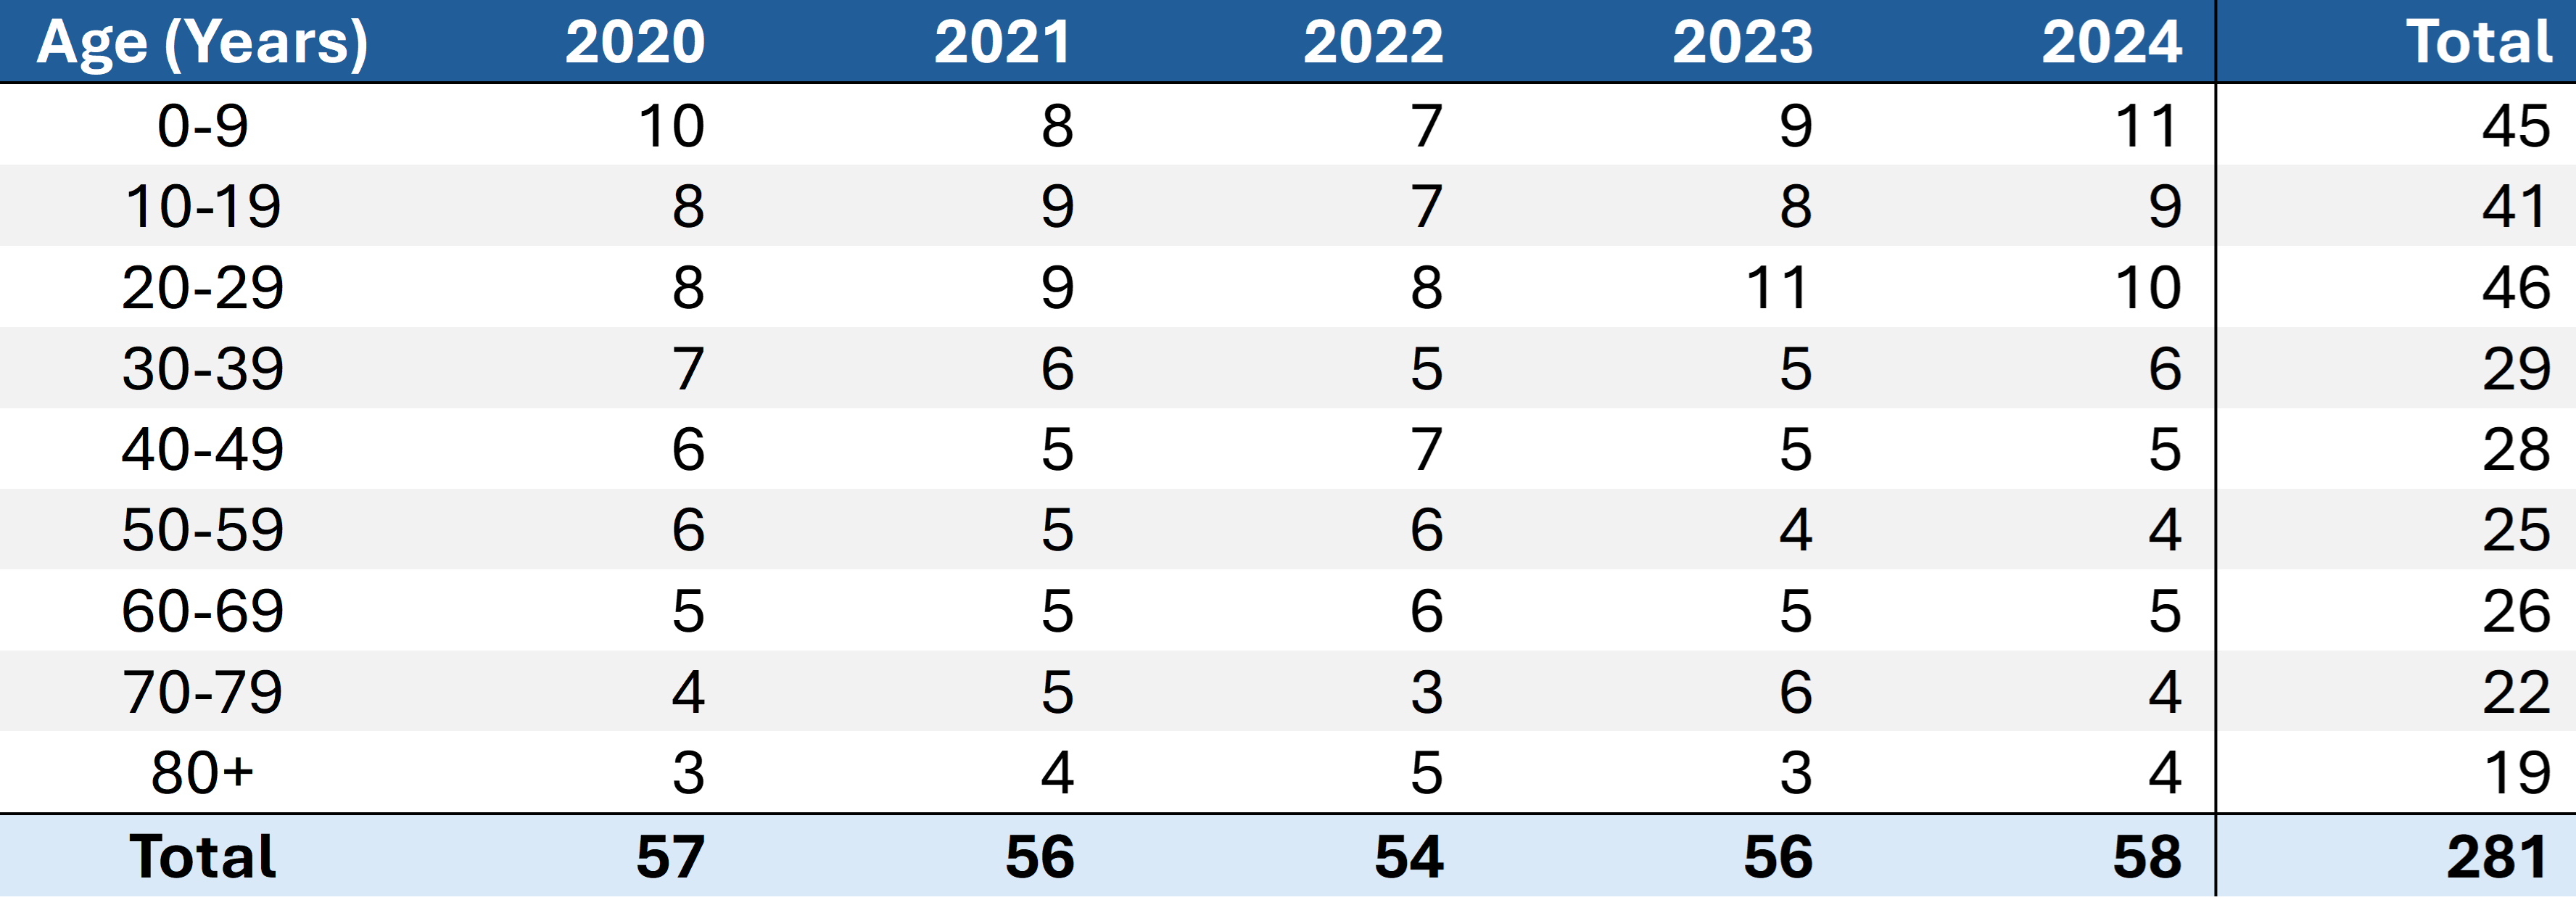
\includegraphics[width=0.95\textwidth]{data_analysis/tables/age_table_example.png}
    \end{tabular}
\end{table}


% =============================================================================
\section{Discussion}
% =============================================================================


% =============================================================================
\section{Limitations}
% =============================================================================


% =============================================================================
\section{Conclusion}
% =============================================================================


% =============================================================================
\clearpage
\section{Recommendations}
% =============================================================================

% Each recommendation should name the responsible party in bold italics.
\textit{\textbf{Responsible: [Unit/team name]}}

Recommendation text here.


% =============================================================================
% REFERENCES — do not edit these two lines
% =============================================================================
\clearpage
\addcontentsline{toc}{section}{References}
\printbibliography[heading=subbibliography, title={References}]


% =============================================================================
% APPENDICES
% Uncomment the section(s) relevant to this chapter.
% Upload your files to data_analysis/appendices/ before including them.
% REMOVE the entire subappendices block if this chapter has no appendices.
% =============================================================================
\begin{subappendices}

% HOW TO INCLUDE A PDF APPENDIX
% Each page of your PDF is included as a separate \includegraphics line.
% Add or remove \includegraphics lines to match the number of pages in your file.
% Upload your PDF to the data_analysis/appendices/ folder before compiling.
% Tip: avoid spaces in filenames — use underscores instead (e.g. my_factsheet.pdf).

% --- LAY SUMMARY / FACTSHEET ---
\clearpage
\section{Lay summary}
\label{app:lay_summary}
\nopagebreak
\centering

\includegraphics[page=1, width=\textwidth]{data_analysis/appendices/factsheet.pdf}
% Add more \includegraphics lines here for additional pages
\RaggedRight

% --- CONFERENCE PRESENTATION SLIDES ---
% \clearpage
% \section{Conference presentation slides}
% \label{app:presentation}
% \nopagebreak
% \centering
% \includegraphics[page=1,width=\textwidth]{data_analysis/appendices/presentation.pdf}
% \clearpage
% \includegraphics[page=2,width=\textwidth]{data_analysis/appendices/presentation.pdf}
% % Add more \includegraphics lines here for additional pages
% \RaggedRight

% --- MANUSCRIPT ---
% \clearpage
% \section{Manuscript}
% \label{app:manuscript}
% \nopagebreak
% \centering
% \includegraphics[page=1,width=\textwidth]{data_analysis/appendices/manuscript.pdf}
% \clearpage
% \includegraphics[page=2,width=\textwidth]{data_analysis/appendices/manuscript.pdf}
% % Add more \includegraphics lines here for additional pages
% \RaggedRight

\end{subappendices}

% =============================================================================
% CHAPTER 3: SURVEILLANCE SYSTEM PROJECT (Major competency 2)
% =============================================================================
% Replace "PROJECT TITLE 2" with your project title.
% See INSTRUCTIONS.md for how to add figures, tables, citations, abbreviations.
% =============================================================================

\chapter{PROJECT TITLE 2}
\label{chap:project_2}
\clearpage

\setcounter{tocdepth}{5}
\setcounter{secnumdepth}{4}
\etocdepthtag.toc{mtchapter}

\localtoc
\clearpage

% LOCAL LIST OF TABLES — remove this line if this chapter has no tables
\locallistoftables
% LOCAL LIST OF FIGURES — remove this line if this chapter has no figures
\locallistoffigures
\clearpage

\glsresetall[abbreviations]


% =============================================================================
\section{Prologue}
% =============================================================================

\subsection{Study rationale}

\subsection{My role}

\subsection{Lessons learnt}

\subsection{Public health impact}

\subsection{MAE competencies addressed}
\begin{itemize}
    \item Establish a surveillance system or health information system
    \item Teaching field epidemiology
\end{itemize}

\subsection{Acknowledgements}


% =============================================================================
\glsresetall[abbreviations]
\clearpage
\section{Abstract}
% =============================================================================

\subsection*{Objective}

\subsection*{Methods}

\subsection*{Results}

\subsection*{Conclusion}


% =============================================================================
\glsresetall[abbreviations]
\clearpage
\section{Introduction}
% =============================================================================


% =============================================================================
\section{Methods}
% =============================================================================

\subsection{Ethics}


% =============================================================================
\section{Results}
% =============================================================================
% HOW TO ADD A FIGURE (save image to surveillance/figures/):
%
%   \begin{figure}[H]
%       \centering
%       \includegraphics[width=0.85\textwidth]{surveillance/figures/my_figure.png}
%       \caption{Caption goes BELOW the figure.}
%       \label{fig:my_figure}
%   \end{figure}
%   Reference in text: \cref{fig:my_figure}  →  "Figure 1"
%
% HOW TO ADD A TABLE (save image to surveillance/tables/):
%
%   \begin{table}[H]
%       \caption{Caption goes ABOVE the table.}
%       \label{tab:my_table}
%       \centering
%       \begin{tabular}{c}
%           \includegraphics[width=0.95\textwidth]{surveillance/tables/my_table.png}
%       \end{tabular}
%   \end{table}
%   Reference in text: \cref{tab:my_table}  →  "Table 1"

% Example figure (replace with your own image and caption):
As shown in \cref{fig:example}, ...

\begin{figure}[H]
    \centering
    
\includegraphics[width=0.85\textwidth]{surveillance/figures/kitkat.png}
    \caption{Example figure caption.}
    \label{fig:example}
\end{figure}


% =============================================================================
\section{Discussion}
% =============================================================================
This is another example of a reference \cite{australian_bureau_of_statistics_standard_2024}. If the chapter does not have a reference there will be a warning in the overleaf log, just ignore it if you don't need one :)

% =============================================================================
\section{Limitations}
% =============================================================================


% =============================================================================
\section{Conclusion}
% =============================================================================


% =============================================================================
\clearpage
\section{Recommendations}
% =============================================================================

% Each recommendation should name the responsible party in bold italics.
\textit{\textbf{Responsible: [Unit/team name]}}

Recommendation text here.


% =============================================================================
% REFERENCES — do not edit these two lines
% =============================================================================
\clearpage
\addcontentsline{toc}{section}{References}
\printbibliography[heading=subbibliography, title={References}]


% =============================================================================
% APPENDICES
% Uncomment the section(s) relevant to this chapter.
% Upload your files to surveillance/appendices/ before including them.
% REMOVE the entire subappendices block if this chapter has no appendices.
% =============================================================================
\begin{subappendices}

% HOW TO INCLUDE A PDF APPENDIX
% Each page of your PDF is included as a separate \includegraphics line.
% Add or remove \includegraphics lines to match the number of pages in your file.
% Upload your PDF to the surveillance/appendices/ folder before compiling.
% Tip: avoid spaces in filenames — use underscores instead (e.g. my_factsheet.pdf).

% --- LAY SUMMARY / FACTSHEET ---
% \clearpage
% \section{Lay summary}
% \label{app:lay_summary}
% \nopagebreak
% \centering
% \includegraphics[page=1,width=\textwidth]{surveillance/appendices/lay_summary.pdf}
% \clearpage
% \includegraphics[page=2,width=\textwidth]{surveillance/appendices/lay_summary.pdf}
% % Add more \includegraphics lines here for additional pages
% \RaggedRight

% --- CONFERENCE PRESENTATION SLIDES ---
% \clearpage
% \section{Conference presentation slides}
% \label{app:presentation}
% \nopagebreak
% \centering
% \includegraphics[page=1,width=\textwidth]{surveillance/appendices/presentation.pdf}
% \clearpage
% \includegraphics[page=2,width=\textwidth]{surveillance/appendices/presentation.pdf}
% % Add more \includegraphics lines here for additional pages
% \RaggedRight

% --- MANUSCRIPT ---
% \clearpage
% \section{Manuscript}
% \label{app:manuscript}
% \nopagebreak
% \centering
% \includegraphics[page=1,width=\textwidth]{surveillance/appendices/manuscript.pdf}
% \clearpage
% \includegraphics[page=2,width=\textwidth]{surveillance/appendices/manuscript.pdf}
% % Add more \includegraphics lines here for additional pages
% \RaggedRight

\end{subappendices}

% =============================================================================
% CHAPTER 4: EPIDEMIOLOGICAL STUDY (Major competency 3)
% =============================================================================
% Replace "PROJECT TITLE 3" with your project title.
% See INSTRUCTIONS.md for how to add figures, tables, citations, abbreviations.
% =============================================================================

\chapter{PROJECT TITLE 3}
\label{chap:project_3}
\clearpage

\setcounter{tocdepth}{5}
\setcounter{secnumdepth}{4}
\etocdepthtag.toc{mtchapter}

\localtoc
\clearpage

% LOCAL LIST OF TABLES — remove this line if this chapter has no tables
\locallistoftables
% LOCAL LIST OF FIGURES — remove this line if this chapter has no figures
\locallistoffigures
\clearpage

\glsresetall[abbreviations]


% =============================================================================
\section{Prologue}
% =============================================================================

\subsection{Study rationale}

\subsection{My role}

\subsection{Lessons learnt}

\subsection{Public health impact}

\subsection{MAE competencies addressed}
\begin{itemize}
  \item Design and conduct an epidemiological study
  \item Literature review
\end{itemize}

\subsection{Acknowledgements}


% =============================================================================
\glsresetall[abbreviations]
\clearpage
\section{Abstract}
% =============================================================================

\subsection*{Objectives}

\subsection*{Methods}

\subsection*{Results}

\subsection*{Conclusion}


% =============================================================================
\glsresetall[abbreviations]
\clearpage
\section{Introduction}
% =============================================================================
This is another random reference \cite{centres_for_disease_control_and_prevention_about_2024-1}.

\subsection{Study aim}

\subsection{Study objectives}


% =============================================================================
\section{Methods}
% =============================================================================

\subsection{Study period and population}

\subsection{Case definition}

\subsection{Data collection}

\subsection{Study design}

\subsection{Study outcomes}

\subsection{Exposure variables}

\subsection{Data cleaning}

\subsection{Statistical analyses}

\subsection{Ethics}


% =============================================================================
\section{Results}
% =============================================================================
% HOW TO ADD A TABLE (save image to epistudy/tables/):
%
%   \begin{table}[H]
%       \caption{Caption goes ABOVE the table.}
%       \label{tab:my_table}
%       \centering
%       \begin{tabular}{c}
%           \includegraphics[width=0.95\textwidth]{epistudy/tables/my_table.png}
%       \end{tabular}
%   \end{table}
%   Reference in text: \cref{tab:my_table}  →  "Table 1"
%
% HOW TO ADD A FIGURE (save image to epistudy/figures/):
%
%   \begin{figure}[H]
%       \centering
%       \includegraphics[width=0.85\textwidth]{epistudy/figures/my_figure.png}
%       \caption{Caption goes BELOW the figure.}
%       \label{fig:my_figure}
%   \end{figure}
%   Reference in text: \cref{fig:my_figure}  →  "Figure 1"


% =============================================================================
\section{Discussion}
% =============================================================================


% =============================================================================
\section{Limitations}
% =============================================================================


% =============================================================================
\section{Conclusion}
% =============================================================================


% =============================================================================
\clearpage
\section{Recommendations}
% =============================================================================

% Each recommendation should name the responsible party in bold italics.
\textit{\textbf{Responsible: [Unit/team name]}}

Recommendation text here.


% =============================================================================
% REFERENCES — do not edit these two lines
% =============================================================================
\clearpage
\addcontentsline{toc}{section}{References}
\printbibliography[heading=subbibliography, title={References}]


% =============================================================================
% APPENDICES
% Uncomment the section(s) relevant to this chapter.
% Upload your files to epistudy/appendices/ before including them.
% REMOVE the entire subappendices block if this chapter has no appendices.
% =============================================================================
\begin{subappendices}

% HOW TO INCLUDE A PDF APPENDIX
% Each page of your PDF is included as a separate \includegraphics line.
% Add or remove \includegraphics lines to match the number of pages in your file.
% Upload your PDF to the epistudy/appendices/ folder before compiling.
% Tip: avoid spaces in filenames — use underscores instead (e.g. my_factsheet.pdf).

% --- LAY SUMMARY / FACTSHEET ---
% \clearpage
% \section{Lay summary}
% \label{app:lay_summary}
% \nopagebreak
% \centering
% \includegraphics[page=1,width=\textwidth]{epistudy/appendices/lay_summary.pdf}
% \clearpage
% \includegraphics[page=2,width=\textwidth]{epistudy/appendices/lay_summary.pdf}
% % Add more \includegraphics lines here for additional pages
% \RaggedRight

% --- CONFERENCE PRESENTATION SLIDES ---
% \clearpage
% \section{Conference presentation slides}
% \label{app:presentation}
% \nopagebreak
% \centering
% \includegraphics[page=1,width=\textwidth]{epistudy/appendices/presentation.pdf}
% \clearpage
% \includegraphics[page=2,width=\textwidth]{epistudy/appendices/presentation.pdf}
% % Add more \includegraphics lines here for additional pages
% \RaggedRight

% --- MANUSCRIPT ---
% \clearpage
% \section{Manuscript}
% \label{app:manuscript}
% \nopagebreak
% \centering
% \includegraphics[page=1,width=\textwidth]{epistudy/appendices/manuscript.pdf}
% \clearpage
% \includegraphics[page=2,width=\textwidth]{epistudy/appendices/manuscript.pdf}
% % Add more \includegraphics lines here for additional pages
% \RaggedRight

\end{subappendices}

% =============================================================================
% CHAPTER 5: OUTBREAK INVESTIGATION (Major competency 4)
% =============================================================================
% Replace "PROJECT TITLE 4" with your outbreak report title.
% See INSTRUCTIONS.md for how to add figures, tables, citations, abbreviations.
% =============================================================================

\chapter{PROJECT TITLE 4}
\label{chap:project_4}
\clearpage

\setcounter{tocdepth}{5}
\setcounter{secnumdepth}{4}
\etocdepthtag.toc{mtchapter}

\localtoc
\clearpage

% LOCAL LIST OF TABLES — remove this line if this chapter has no tables
\locallistoftables
% LOCAL LIST OF FIGURES — remove this line if this chapter has no figures
\locallistoffigures
\clearpage

\glsresetall[abbreviations]


% =============================================================================
\section{Prologue}
% =============================================================================

\subsection{Study rationale}

\subsection{My role}

\subsection{Lessons learnt}

\subsection{Public health impact}

\subsection{MAE competencies addressed}
\begin{itemize}
  \item Investigation of an acute public health problem (outbreak investigation)
  \item Conference presentation
  \item Peer-reviewed publication
\end{itemize}

\subsection{Acknowledgements}


% =============================================================================
\glsresetall[abbreviations]
\clearpage
\section{Abstract}
% =============================================================================

\subsection*{Background}

\subsection*{Methods}

\subsection*{Results}

\subsection*{Conclusion}


% =============================================================================
\glsresetall[abbreviations]
\clearpage
\section{Introduction}
% =============================================================================


% =============================================================================
\section{Methods}
% =============================================================================

\subsection{Epidemiological investigation}

\subsubsection{Data collection}

\subsubsection{Case definition}

\paragraph*{Confirmed case}

\paragraph*{Probable case}

\subsubsection{Data management}

\subsubsection{Data analysis}

\subsubsection{Public health action}

\subsubsection{Communication}


\subsection{Environmental health investigation}


\subsection{Laboratory investigation}

\subsubsection{Clinical samples}

\subsubsection{Environmental samples}

\subsection{Ethics}


% =============================================================================
\section{Results}
% =============================================================================
% HOW TO ADD A FIGURE (e.g. epicurve — save to outbreak/figures/):
%
%   \begin{figure}[H]
%       \centering
%       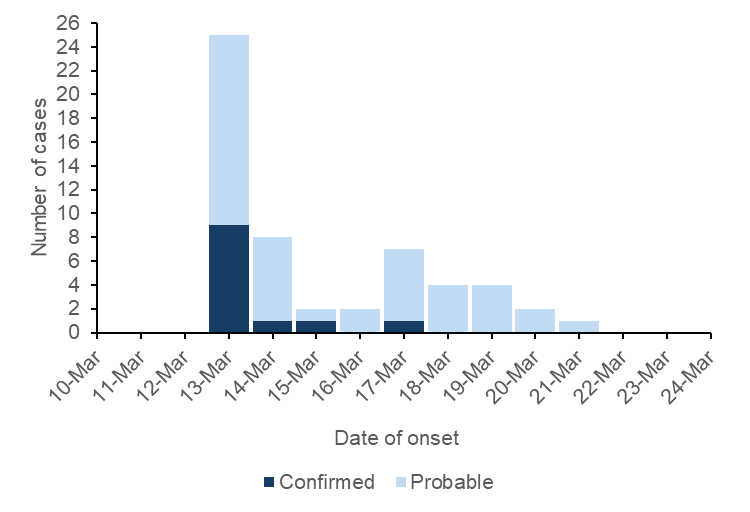
\includegraphics[width=0.95\textwidth]{outbreak/figures/epicurve.png}
%       \caption{Caption goes BELOW the figure.}
%       \label{fig:epicurve}
%   \end{figure}
%   Reference in text: \cref{fig:epicurve}  →  "Figure 1"
%
% HOW TO ADD A TABLE (e.g. attack rate table — save to outbreak/tables/):
%
%   \begin{table}[H]
%       \caption{Caption goes ABOVE the table.}
%       \label{tab:attack_rates}
%       \centering
%       \begin{tabular}{c}
%           \includegraphics[width=0.95\textwidth]{outbreak/tables/attack_rates.png}
%       \end{tabular}
%   \end{table}
%   Reference in text: \cref{tab:attack_rates}  →  "Table 1"

\subsection{Epidemiological investigation}

\subsection{Environmental health investigation}

\subsection{Laboratory investigation}


% =============================================================================
\section{Discussion}
% =============================================================================
Another example of a reference so there's no warnings for this chapter \cite{tasmanian_department_of_health_guidelines_2024}

% =============================================================================
\section{Limitations}
% =============================================================================


% =============================================================================
\section{Conclusion}
% =============================================================================


% =============================================================================
% REFERENCES — do not edit these two lines
% =============================================================================
\clearpage
\addcontentsline{toc}{section}{References}
\printbibliography[heading=subbibliography, title={References}]


% =============================================================================
% APPENDICES
% Uncomment the section(s) relevant to this chapter.
% Upload your files to outbreak/appendices/ before including them.
% REMOVE the entire subappendices block if this chapter has no appendices.
% =============================================================================
\begin{subappendices}

% HOW TO INCLUDE A PDF APPENDIX
% Each page of your PDF is included as a separate \includegraphics line.
% Add or remove \includegraphics lines to match the number of pages in your file.
% Upload your PDF to the outbreak/appendices/ folder before compiling.
% Tip: avoid spaces in filenames — use underscores instead (e.g. my_slides.pdf).

% --- CONFERENCE PRESENTATION SLIDES ---
\clearpage
\section{Conference presentation slides}
\label{app:presentation}
\nopagebreak
\centering

\includegraphics[page=1,width=\textwidth]{outbreak/appendices/Conference presentation slides.pdf}
\clearpage

\includegraphics[page=2,width=\textwidth]{outbreak/appendices/Conference presentation slides.pdf}
% Add more \includegraphics lines here for additional pages
\RaggedRight

% --- MANUSCRIPT ---
\clearpage
\section{Manuscript}
\label{app:manuscript}
\nopagebreak
\centering

\includegraphics[page=1,width=\textwidth]{outbreak/appendices/Manuscript.pdf}
% Add more \includegraphics lines here for additional pages
\RaggedRight

\end{subappendices}

% =============================================================================
% CHAPTER 6: TEACHING AND OTHER FIELD ACTIVITIES (Minor competency)
% =============================================================================
% See INSTRUCTIONS.md for how to add figures, tables, citations, abbreviations.
% =============================================================================

\chapter{Teaching and other field activities}
\label{chap:teaching}
\clearpage

\setcounter{tocdepth}{5}
\setcounter{secnumdepth}{4}
\etocdepthtag.toc{mtchapter}

\localtoc
\clearpage

% LOCAL LIST OF TABLES — remove this line if this chapter has no tables
\locallistoftables
% LOCAL LIST OF FIGURES — remove this line if this chapter has no figures
\locallistoffigures
\clearpage

\glsresetall[abbreviations]


% =============================================================================
\section{Teaching}
% =============================================================================

\subsection{Lessons from the field}

\subsubsection{My role}

\subsubsection{Training}

\subsubsection{Evaluation of training}

\subsubsection{Lessons learnt}
Another random reference... \cite{world_health_organization_syphilis_2024} but this chapter may not need it, so just ignore the warning.

\subsection{Teaching first-year MAE students}

\subsubsection{My role}

\subsubsection{Training}

\subsubsection{Lessons learnt}


% =============================================================================
\section{Other field activities}
% =============================================================================
% Add a \subsection{} for each distinct activity.
% Remove this section if there are no other field activities to report.


% =============================================================================
% REFERENCES — do not edit these two lines
% =============================================================================
\clearpage
\addcontentsline{toc}{section}{References}
\printbibliography[heading=subbibliography, title={References}]


% =============================================================================
% APPENDICES
% Uncomment the section(s) relevant to this chapter.
% Upload your files to teaching/appendices/ before including them.
% REMOVE the entire subappendices block if this chapter has no appendices.
% =============================================================================
\begin{subappendices}

% HOW TO INCLUDE A PDF APPENDIX
% Each page of your PDF is included as a separate \includegraphics line.
% Add or remove \includegraphics lines to match the number of pages in your file.
% Upload your PDF to the teaching/appendices/ folder before compiling.
% Tip: avoid spaces in filenames — use underscores instead (e.g. my_factsheet.pdf).

% --- LAY SUMMARY / FACTSHEET ---
% \clearpage
% \section{Lay summary}
% \label{app:lay_summary}
% \nopagebreak
% \centering
% \includegraphics[page=1,width=\textwidth]{teaching/appendices/lay_summary.pdf}
% \clearpage
% \includegraphics[page=2,width=\textwidth]{teaching/appendices/lay_summary.pdf}
% % Add more \includegraphics lines here for additional pages
% \RaggedRight

% --- CONFERENCE PRESENTATION SLIDES ---
% \clearpage
% \section{Conference presentation slides}
% \label{app:presentation}
% \nopagebreak
% \centering
% \includegraphics[page=1,width=\textwidth]{teaching/appendices/presentation.pdf}
% \clearpage
% \includegraphics[page=2,width=\textwidth]{teaching/appendices/presentation.pdf}
% % Add more \includegraphics lines here for additional pages
% \RaggedRight

% --- MANUSCRIPT ---
% \clearpage
% \section{Manuscript}
% \label{app:manuscript}
% \nopagebreak
% \centering
% \includegraphics[page=1,width=\textwidth]{teaching/appendices/manuscript.pdf}
% \clearpage
% \includegraphics[page=2,width=\textwidth]{teaching/appendices/manuscript.pdf}
% % Add more \includegraphics lines here for additional pages
% \RaggedRight

\end{subappendices}


\end{document}
